% Filename: Results
% Last update: 
%    - created%
%
%%%%%%%%%%%%%%%%%%%%%%%%%%%%%%%%%%%%%%%%%%%%%%%%%%%%%%%%%%%%%%%%%%%%%%

\section{Results}
\label{sec:results}

All SCIRun networks used to generate results will be included in the open-source data set for future use and editing.

\subsection{Segmentation}

In this project a full, detailed head is segmented into different tissue layers to be able to make an inhomogeneous 3D mesh. 

\begin{figure}[H]
\begin{center}
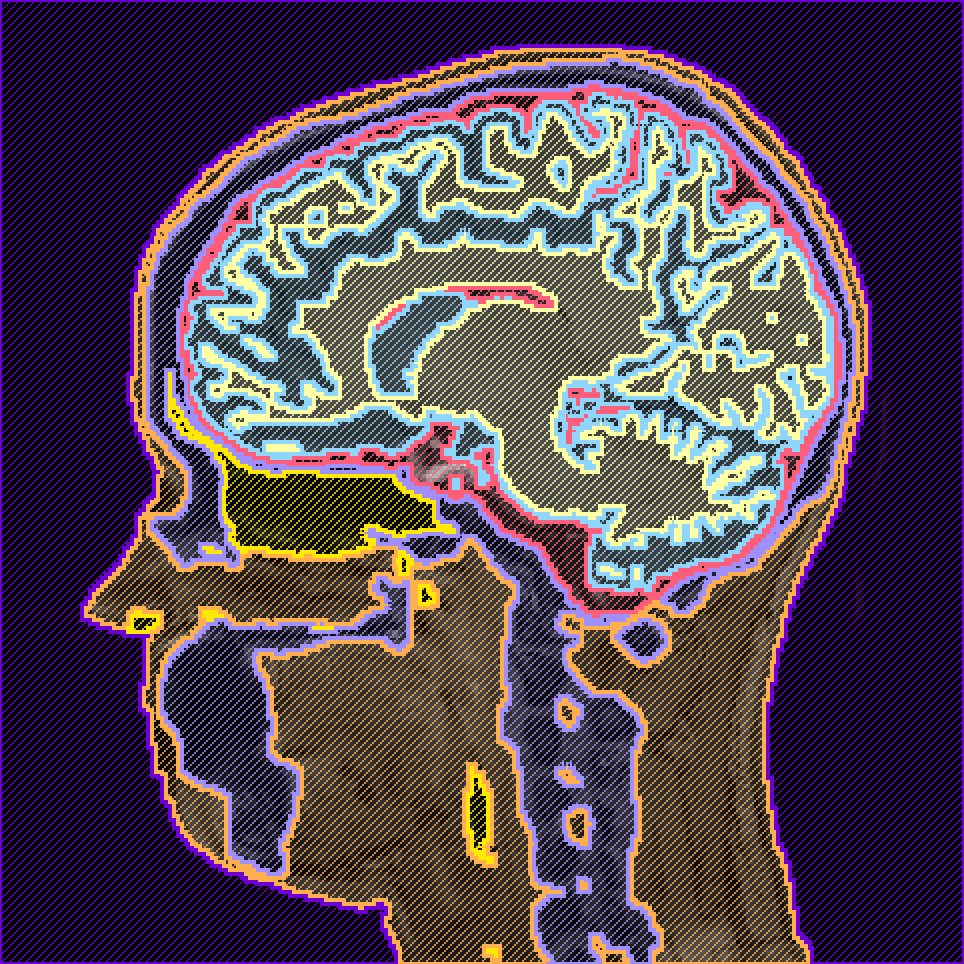
\includegraphics[height=2.35in]{Figures/seg_1}
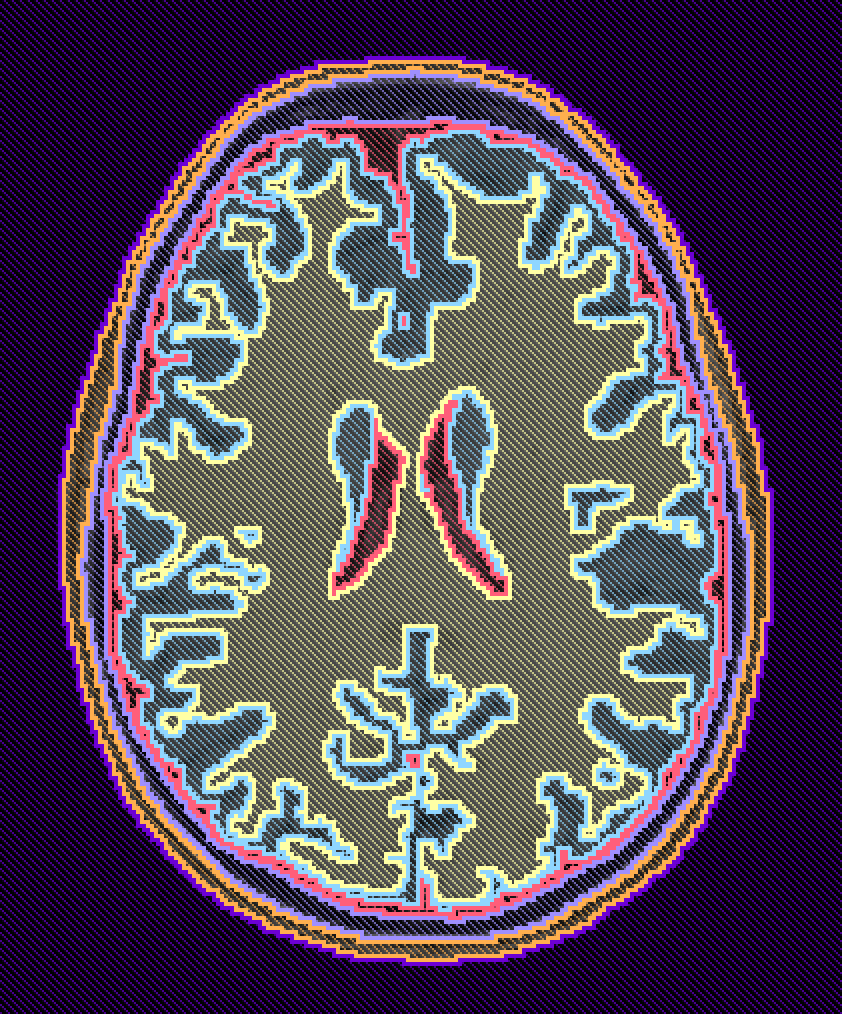
\includegraphics[height=2.35in]{Figures/seg_2}
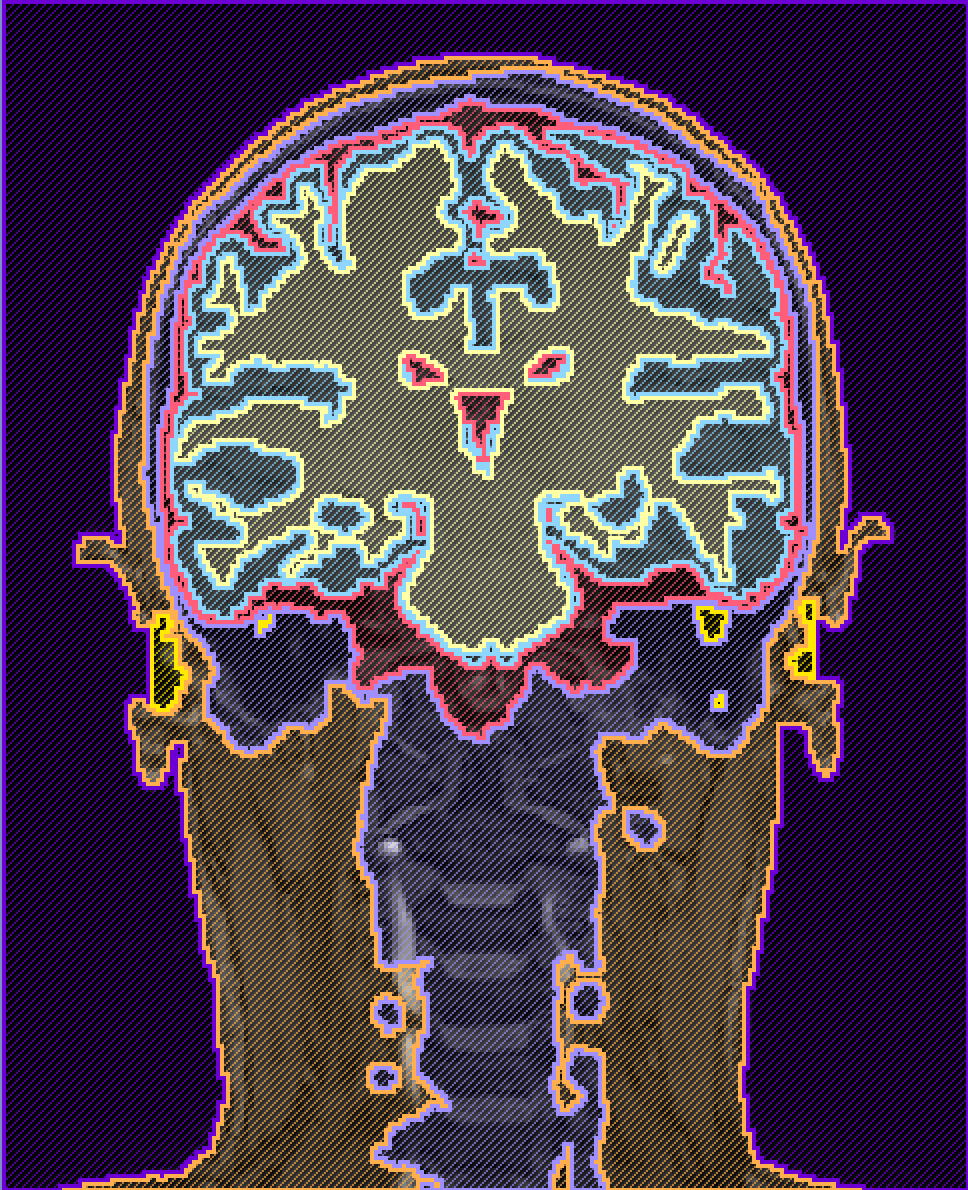
\includegraphics[height=2.35in]{Figures/seg_3}
\caption{A high resolution, eight layer full segmentation made with Seg3D }
\label{fig:fullseg}
\end{center}
\end{figure}

Since there wasn't a CT scan with this data set, the task of segmenting the skull and especially the sinus layers seemed daunting. A basic skull and bone layer was created using FSL skull stripping feature  \cite{ref:bet2} in the brain extraction tool and then concatenated it with a rough bone segmentation using thresholding in Seg3D of black pixels and manually correcting the segmentation. Although a skull and bone segmentation was pieced together, the sinus segmentation seemed extremely difficult and time consuming. After obtaining the pseudo-CT scan, this did not seem like such a large feat anymore. The skull/bone and sinus segmentations made from it fit the brain segmentation extremely well and had no artifacts from combining two different layers together. Although the teeth are solid bone from the subject's permanent retainer.

\begin{figure}[H]
\begin{center}
\includegraphics[width=.49\textwidth]{Figures/skull_before}
\includegraphics[width=.49\textwidth]{Figures/skull_after}
\caption{Skull segmentation comparison: Made with BET \textit{(left)} and made with pseudo-CT \textit{(right). Segmentation was made using Seg3D.}}
\label{fig:skull}
\end{center}
\end{figure}

\begin{figure}[H]
\begin{center}
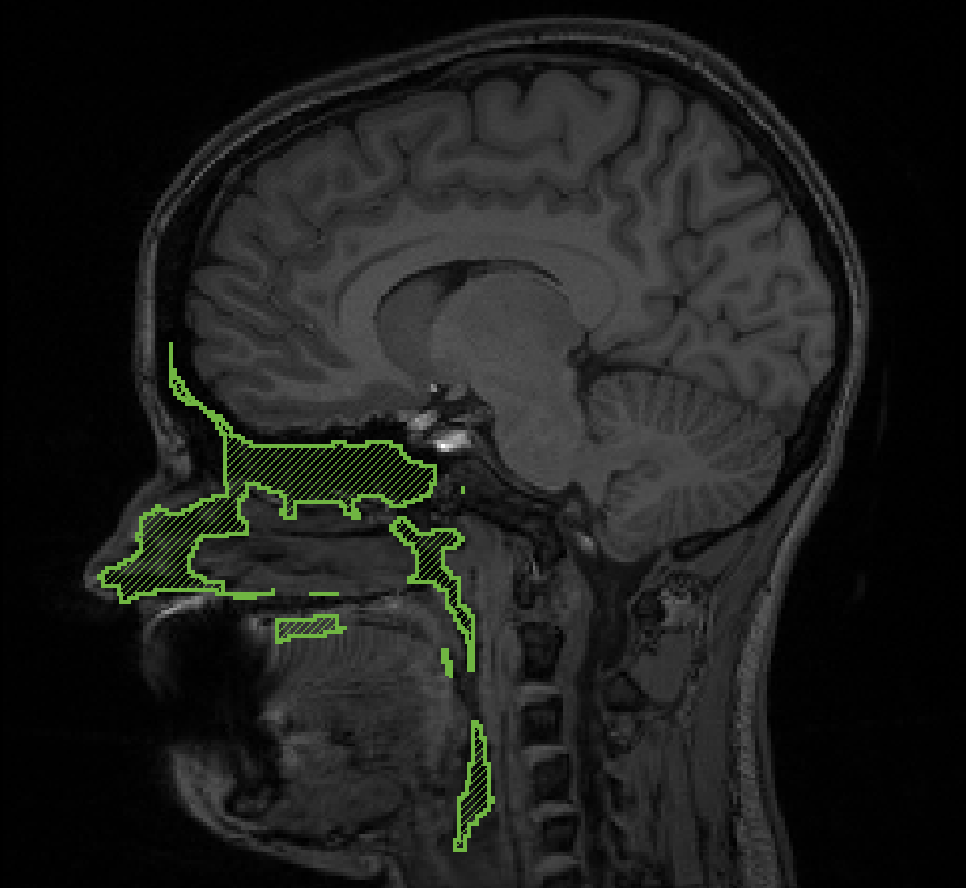
\includegraphics[width=.49\textwidth]{Figures/sinus_sag}
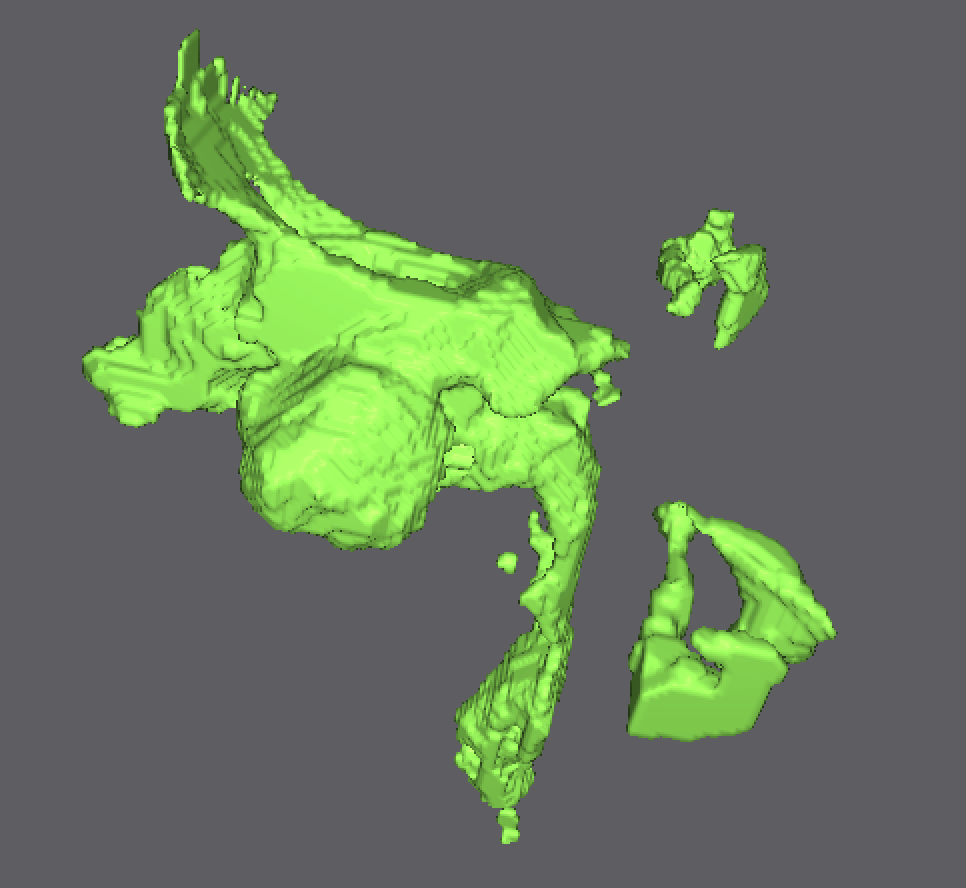
\includegraphics[width=.49\textwidth]{Figures/sinus_iso}
\caption{Sinus segmentation made using Seg3D}
\label{fig:sinus}
\end{center}
\end{figure}

When imaging, the subject is laying on their back which shifts the brain to the back of the head resulting in thin segmented layers in the back of the head. There were also thin layers on the side of the subjects head, the bridge of the nose and the bottom of the chin. These thin layers were made to be at least two pixels thick manually to ensure that a mesh could be made without holes. 

\begin{figure}[H]
\begin{center}
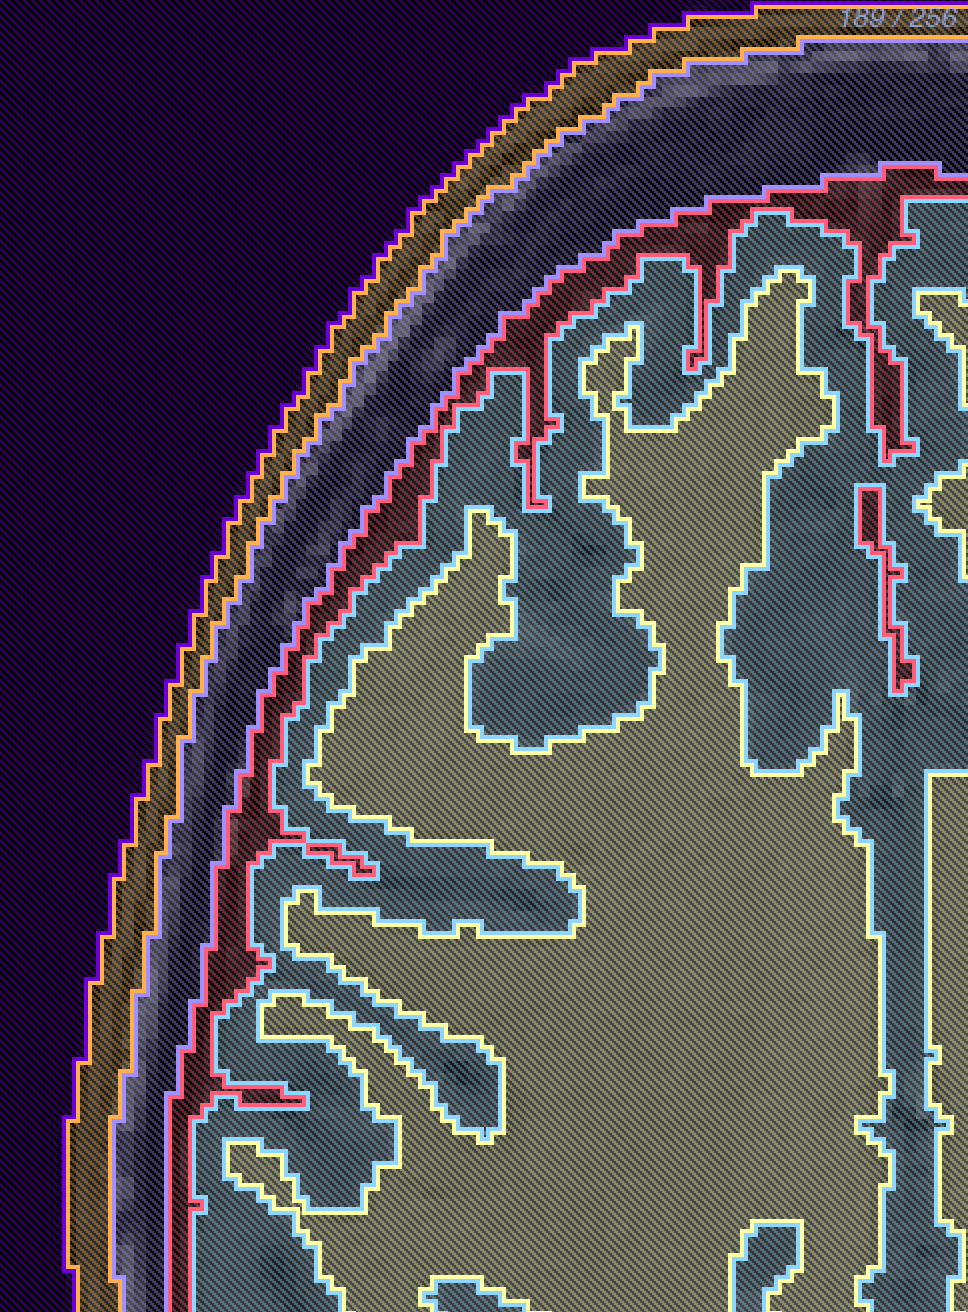
\includegraphics[width=.32\textwidth]{Figures/thin_layer_side}
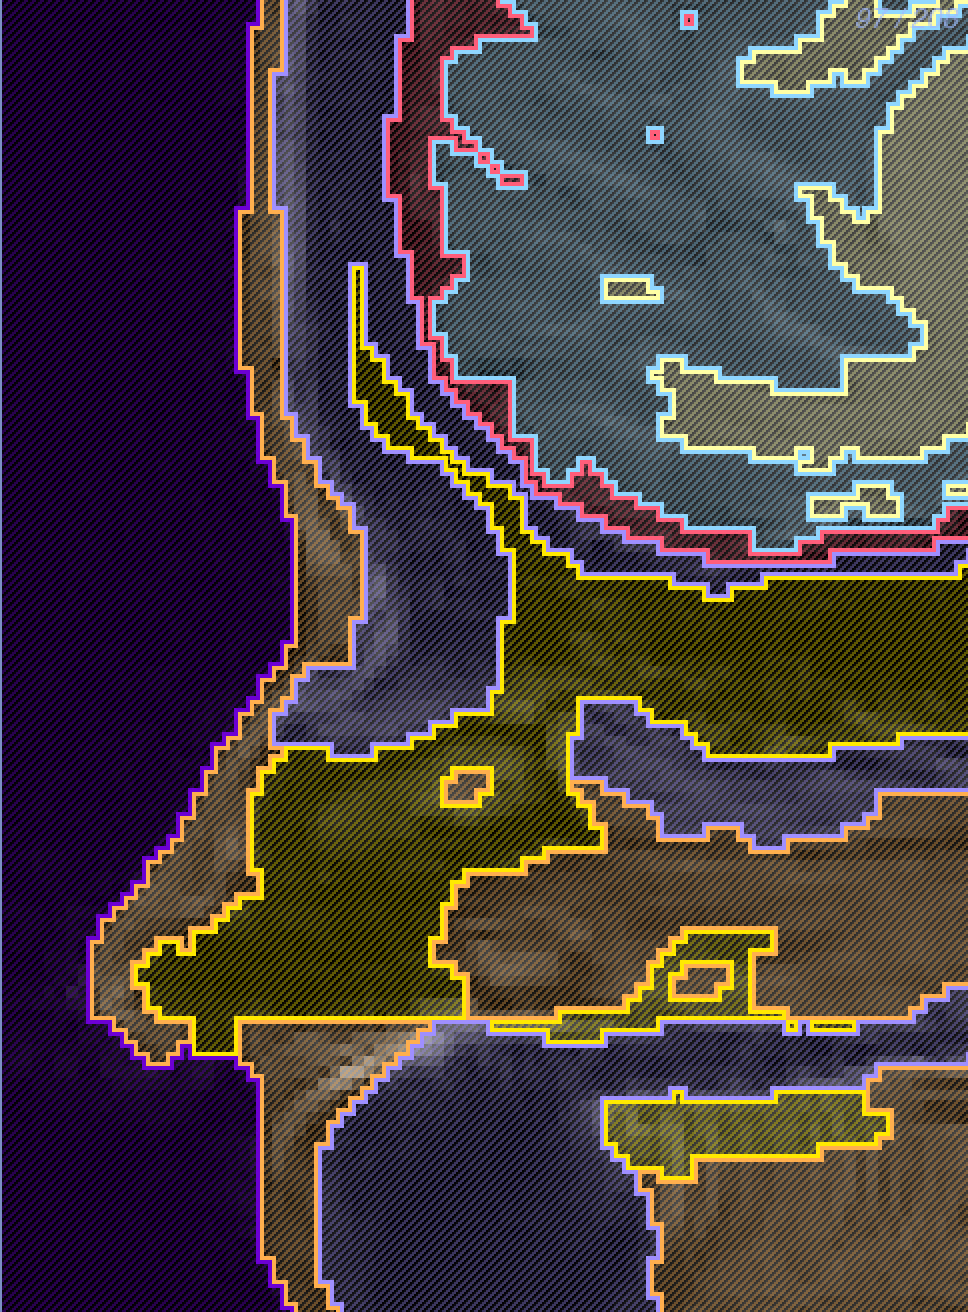
\includegraphics[width=.32\textwidth]{Figures/thin_layer_nose}
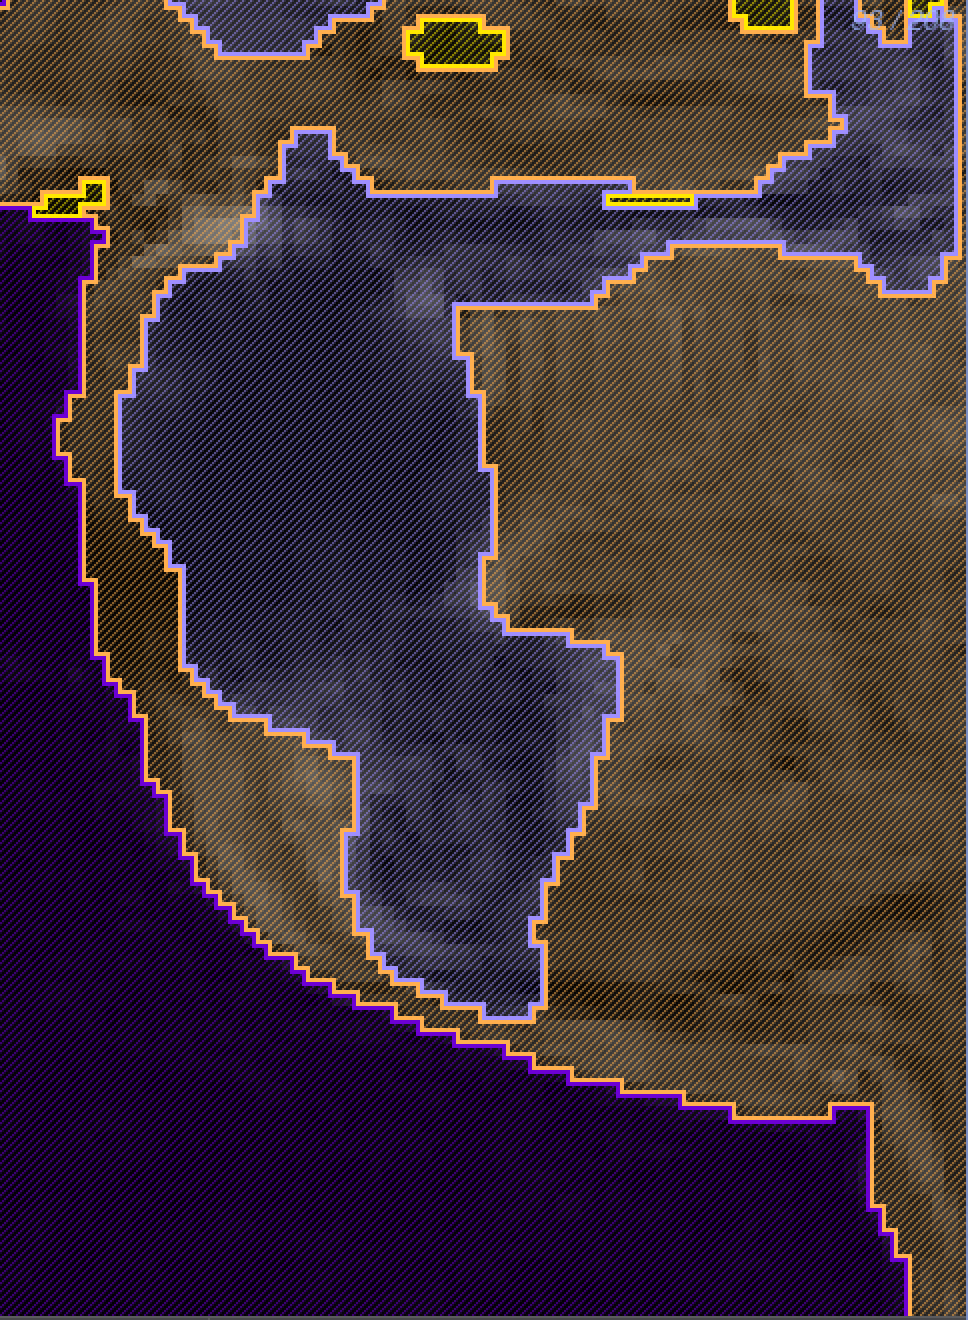
\includegraphics[width=.32\textwidth]{Figures/thin_layer_chin}
\caption{Thin layer segmentations: side of the head \textit{(left)}, bridge of the nose \textit{(middle)}, bottom of the chin \textit{(right)}}
\label{fig:thinseg}
\end{center}
\end{figure}

\subsection{Finite Element Meshes}

The highest resolution mesh, which was made with settings in Section \ref{sec:mesh}, has 60.2 million elements and 10.3 million nodes. This mesh was so large due to the complexity of the segmentation. Simulations run very slow when using this mesh due to its size, and require at least 32GB of RAM in order to not crash SCIRun. 

\begin{figure}[H]
\begin{center}
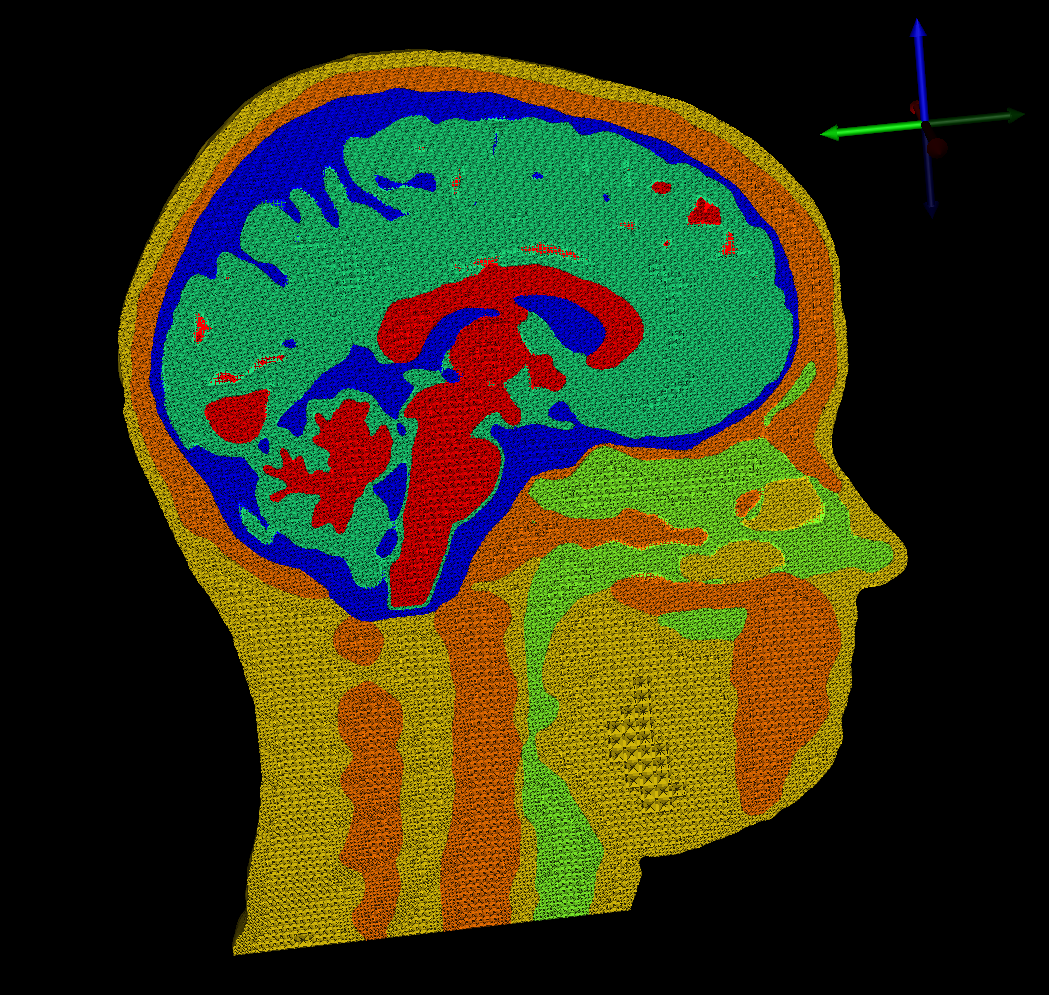
\includegraphics[width=.49\textwidth]{Figures/bigmesh_1}
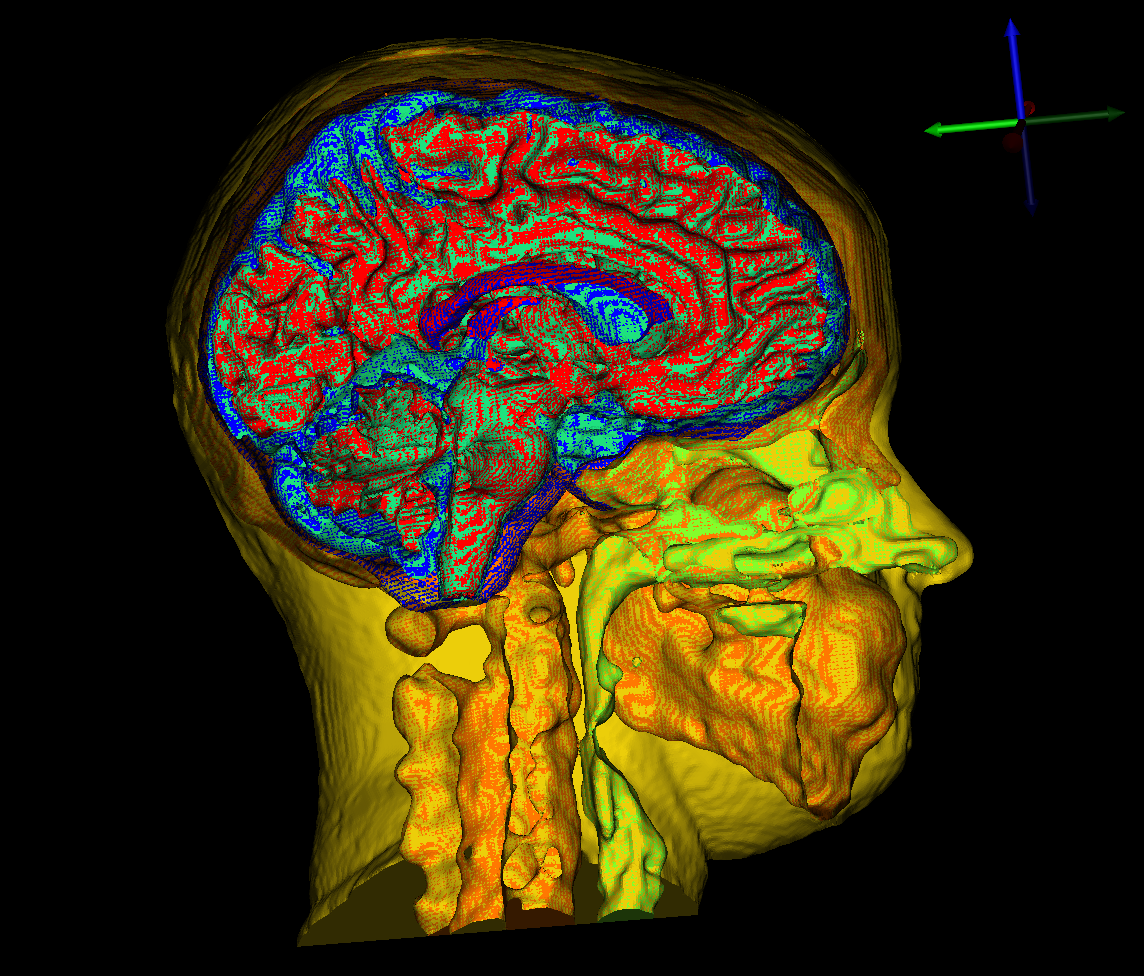
\includegraphics[width=.49\textwidth]{Figures/bigmesh_surface}
\caption{60.2 M element mesh: tetrahedral mesh \textit{(left)}, surface mesh \textit{(right)}}
\label{fig:bigmesh}
\end{center}
\end{figure}

The goal to make smaller meshes was made in order to be able to run simulations more efficiently. After manually changing the sizing field as described in Section \ref{sec:mesh}, a mesh was produced with 15.7 million elements and 2.7 million nodes with no holes. However, this mesh does contain one flat tetrahedra. It is later removed in a SCIRun network, and is currently being investigated by Cleaver software developers.

\begin{figure}[H]
\begin{center}
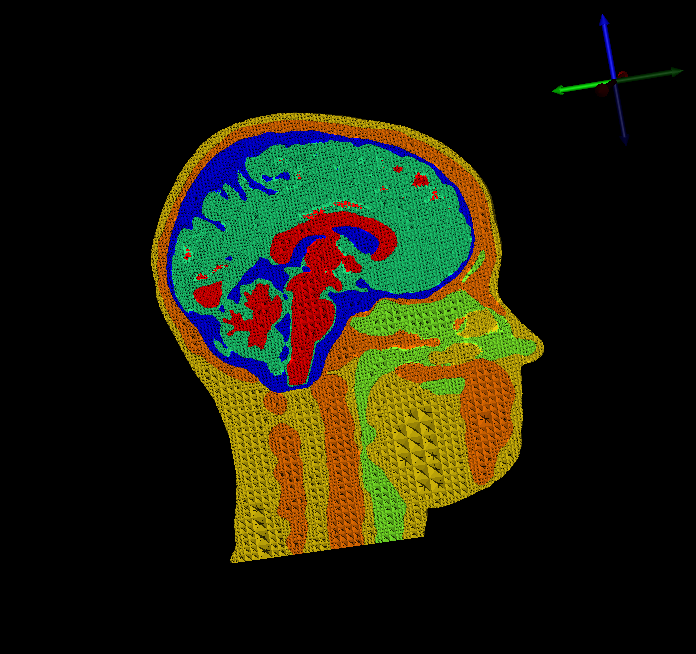
\includegraphics[width=.49\textwidth]{Figures/smallmesh_2}
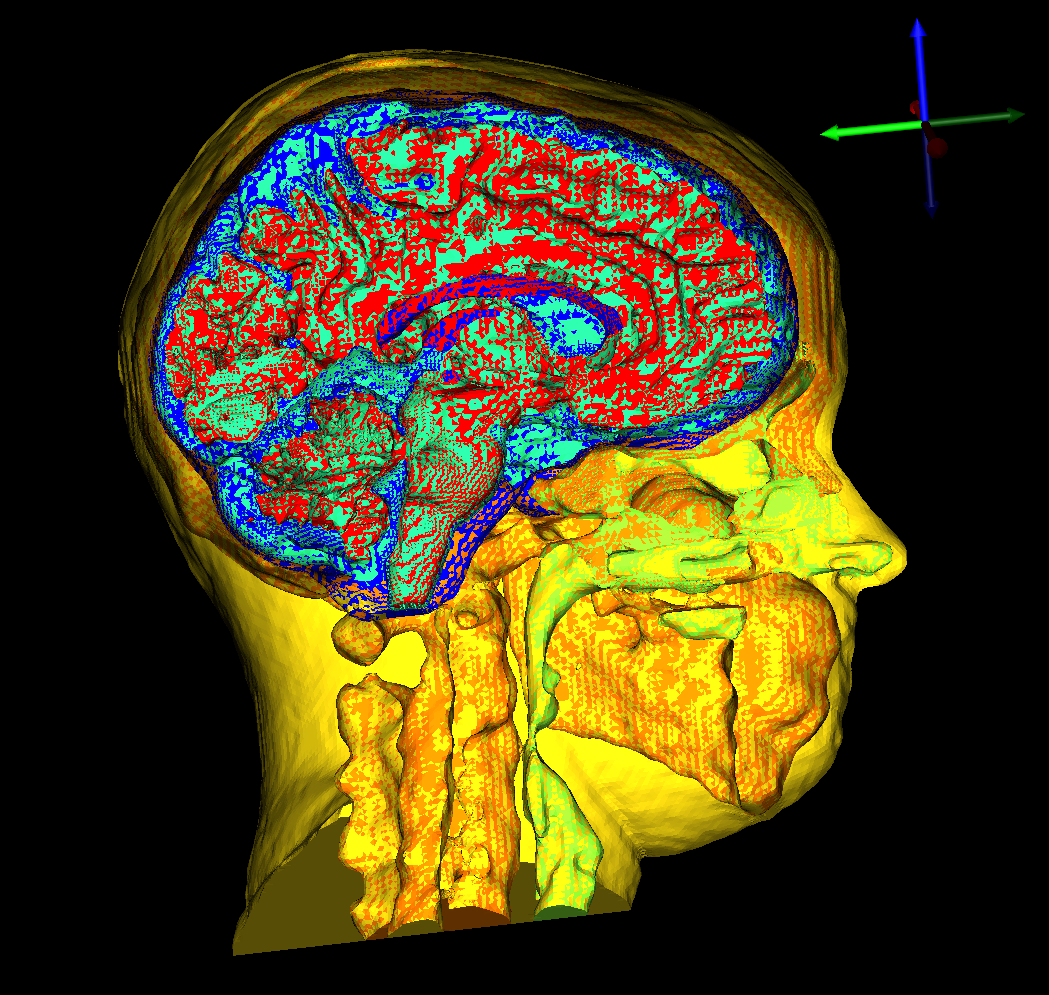
\includegraphics[width=.49\textwidth]{Figures/smallmesh_surface}
\caption{15.7 M element mesh: tetrahedral mesh \textit{(left)}, surface mesh \textit{(right)}}
\label{fig:smallmesh}
\end{center}
\end{figure}

\subsection{Forward Problem}

\subsubsection{Isotropic}

An isotropic, inhomogeneous head model would be expected to have fairly spherical results in propagation of signal. three-dimensional streamlines were generated to show this. Isolines are another way to view this, but in each slice as to better show the differences between isotropic and anisotropic conductivity. Here we can see that the electrodes and dipoles are registered well to the mesh. 

\begin{figure}[H]
\begin{center}
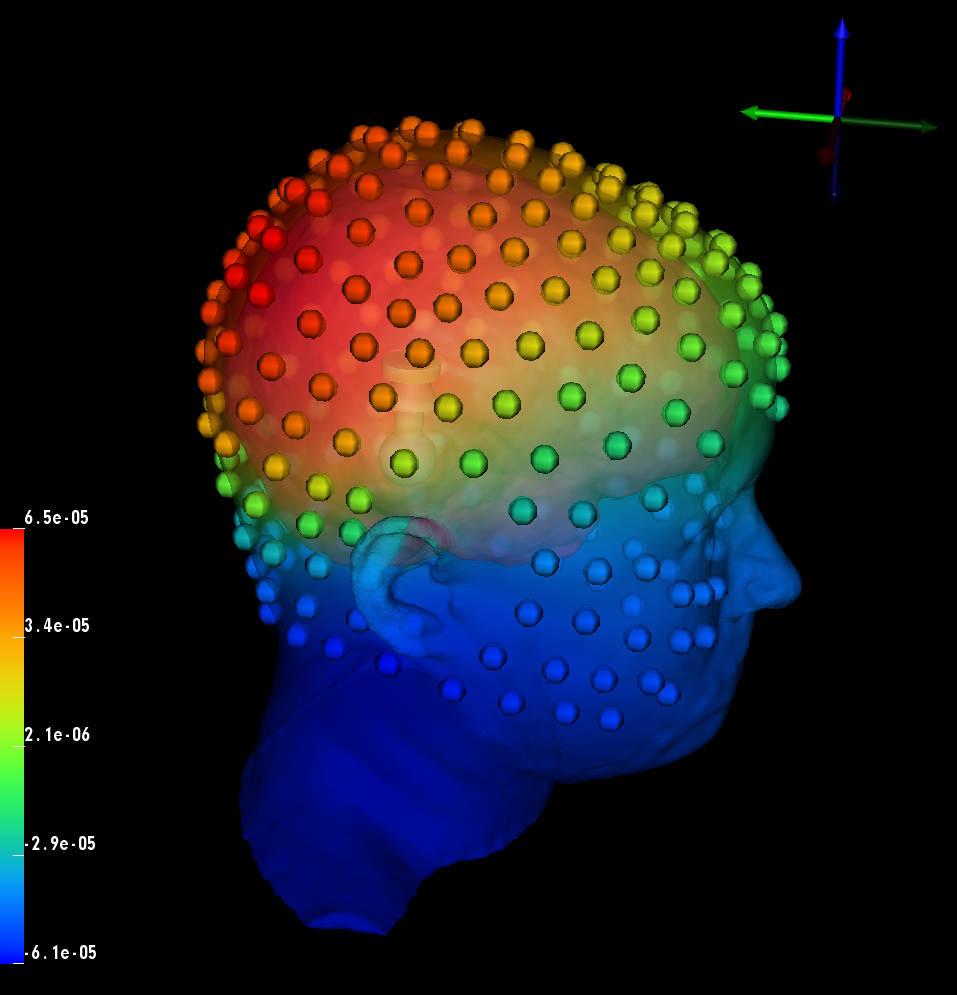
\includegraphics[width=.49\textwidth]{Figures/iso_dipole}
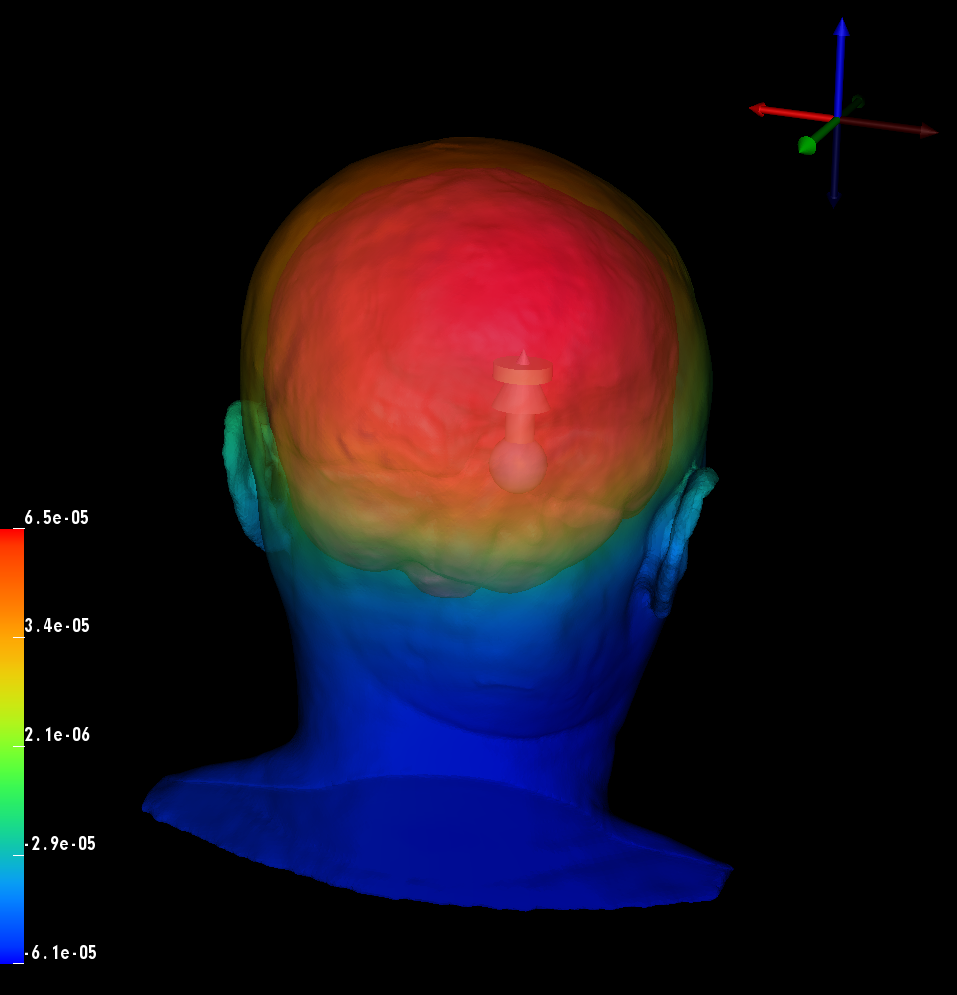
\includegraphics[width=.49\textwidth]{Figures/iso_dipole_2}
\caption{Isotropic forward problem solution with dipole source and data mapped onto the head surface and electrodes.}
\label{fig:isodip}
\end{center}
\end{figure}

\begin{figure}[H]
\begin{center}
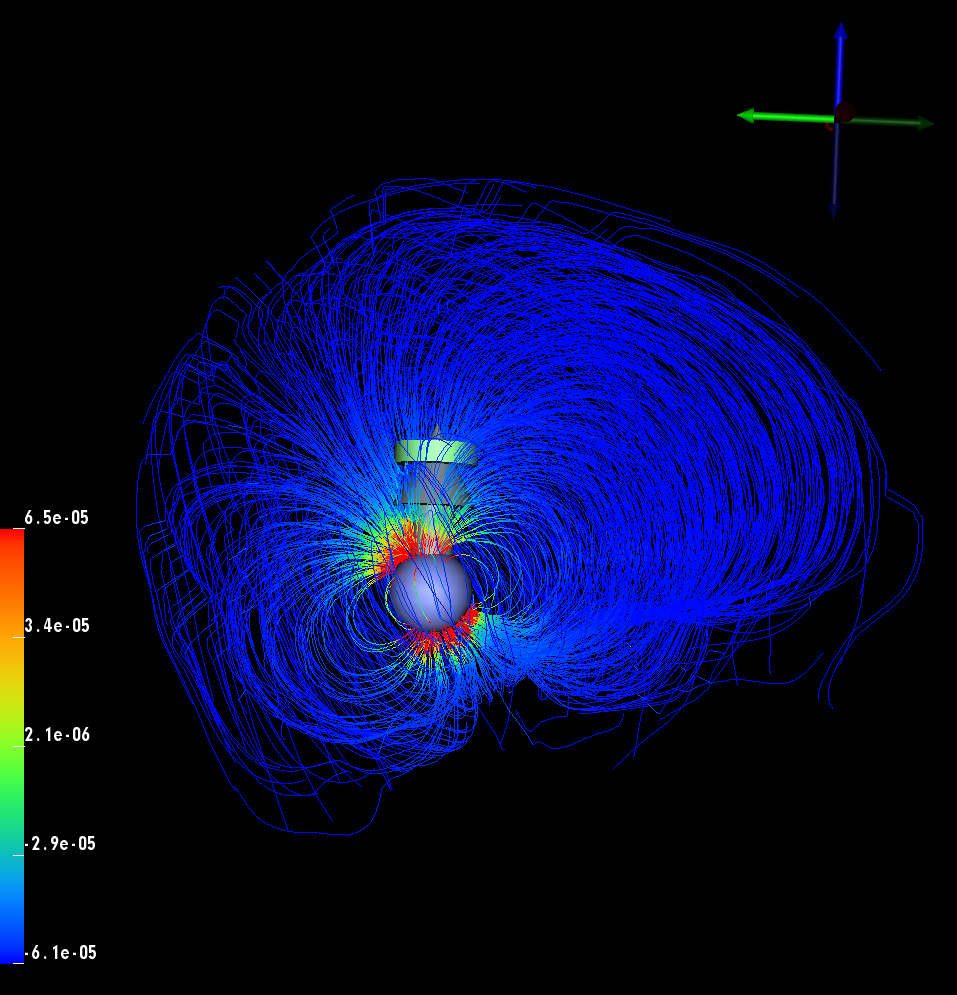
\includegraphics[width=.49\textwidth]{Figures/iso_streamlines}
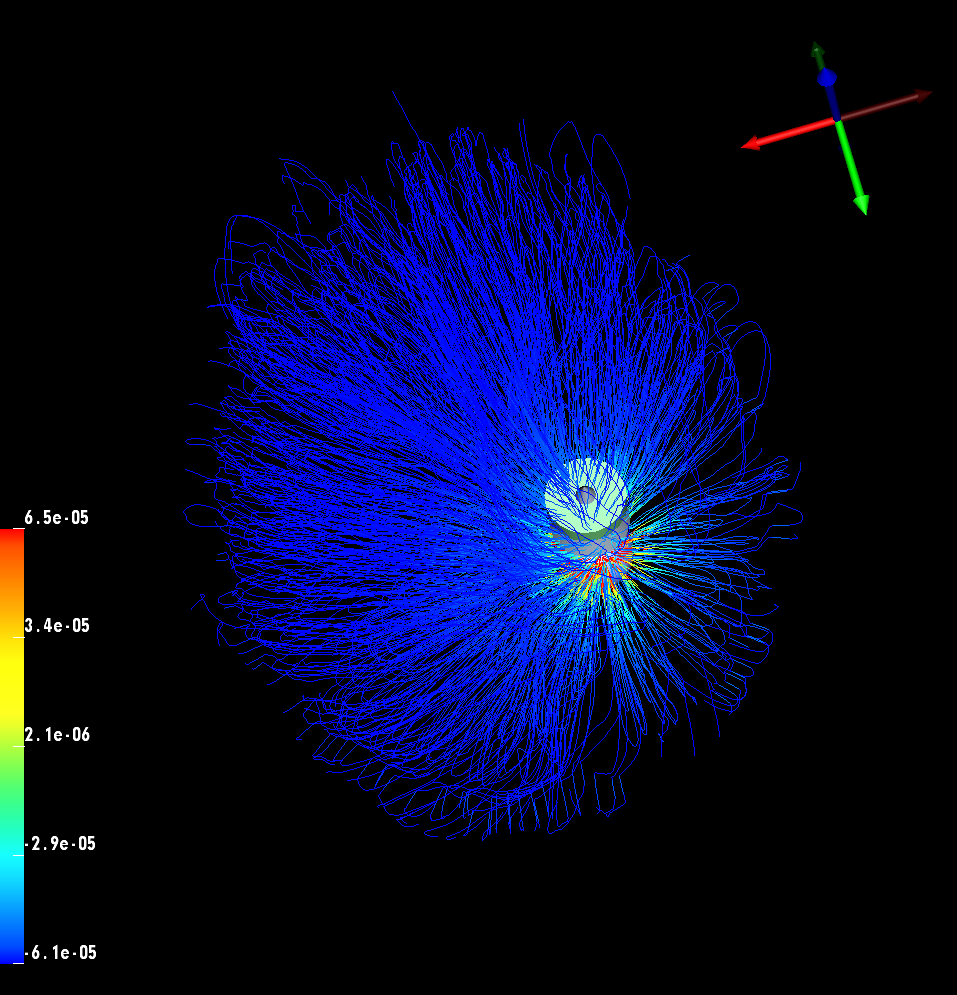
\includegraphics[width=.49\textwidth]{Figures/iso_streamlines_top}
\caption{Isotropic streamlines visualization with dipole source made in SCIRun}
\label{fig:isostream}
\end{center}
\end{figure}

\subsubsection{Anisotropic}

An anisotropic, inhomogeneous head model would be expected to not have spherical results. This can be seen with streamlines, and better so with isolines. As discussed in \ref{sec:cond}, there are two methods of scaling diffusion tensor data. The network has the option to choose one or the other. We can see that the electrodes, the dipoles, and the mesh registered well to the diffusion tensor space.

\begin{figure}[H]
\begin{center}
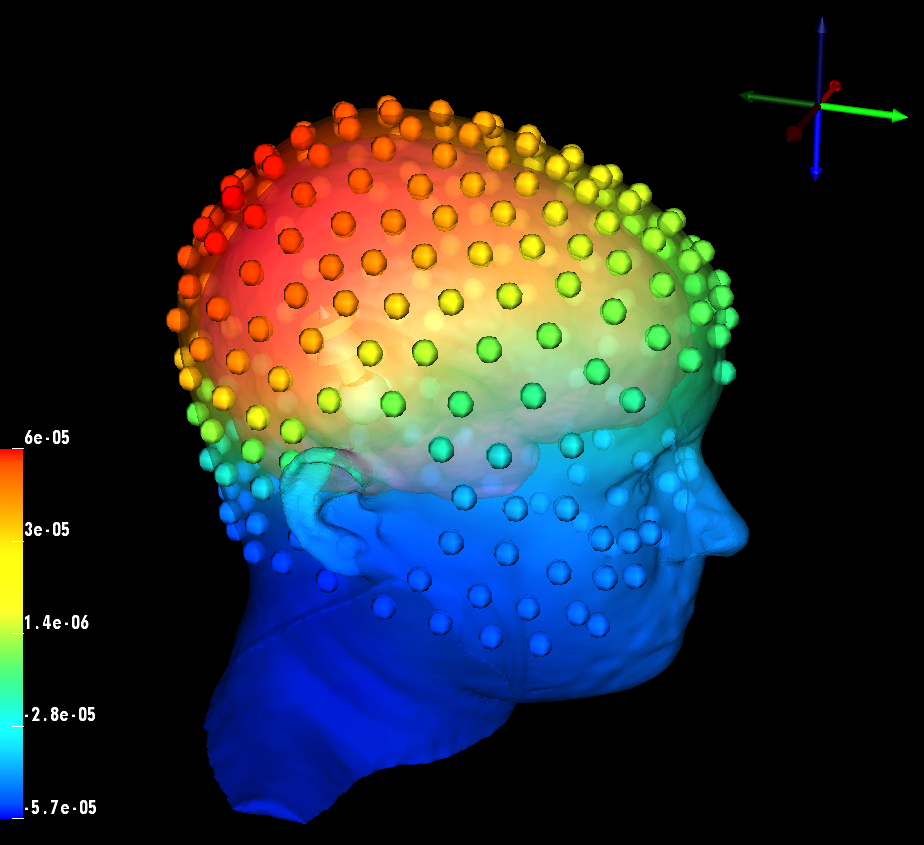
\includegraphics[width=.49\textwidth]{Figures/aniso_dipole}
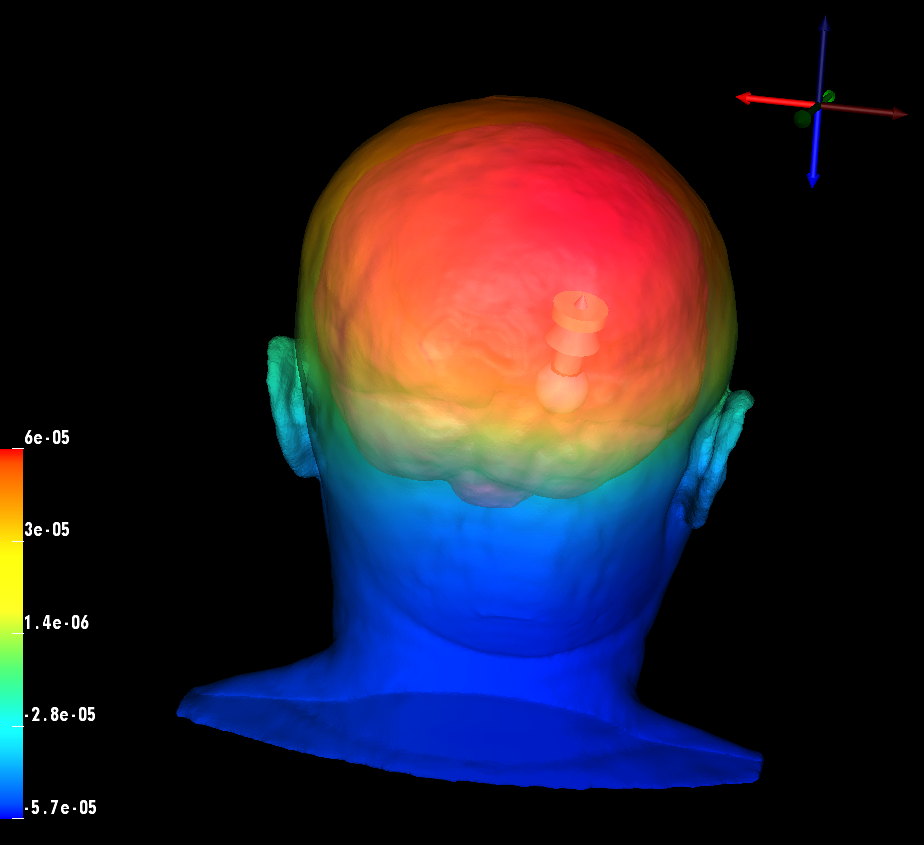
\includegraphics[width=.49\textwidth]{Figures/aniso_dipole_2}
\caption{Anisotropic forward problem solution with dipole source and data mapped onto the head surface and electrodes}
\label{fig:anisodip}
\end{center}
\end{figure}

\begin{figure}[H]
\begin{center}
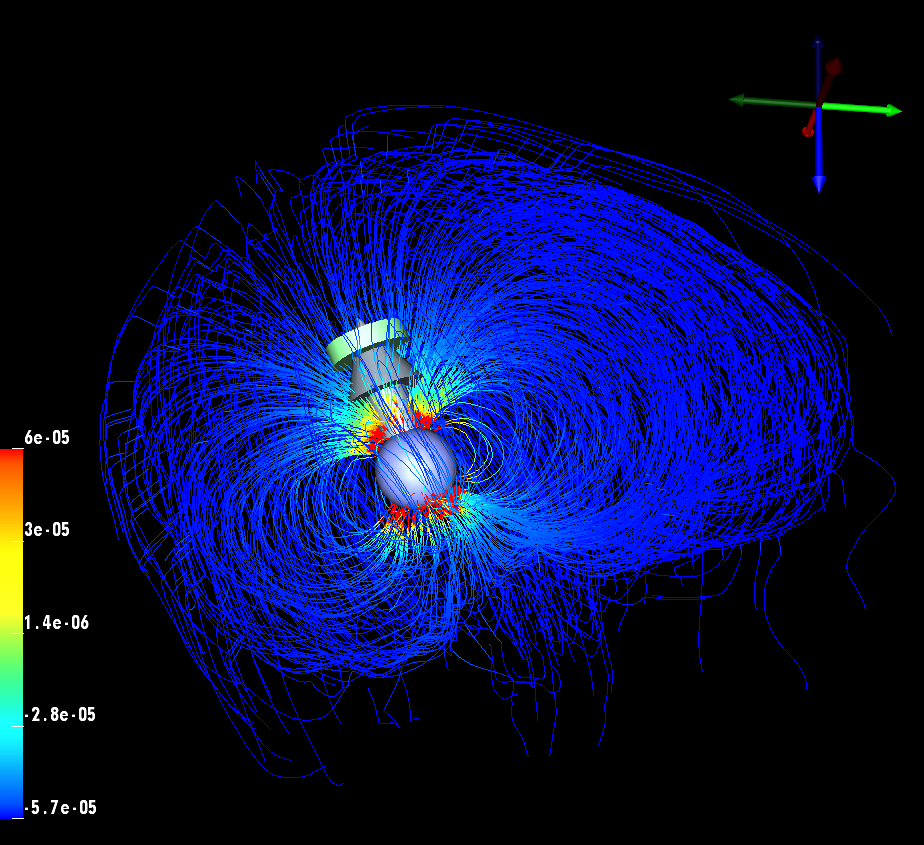
\includegraphics[width=.49\textwidth]{Figures/aniso_streamlines}
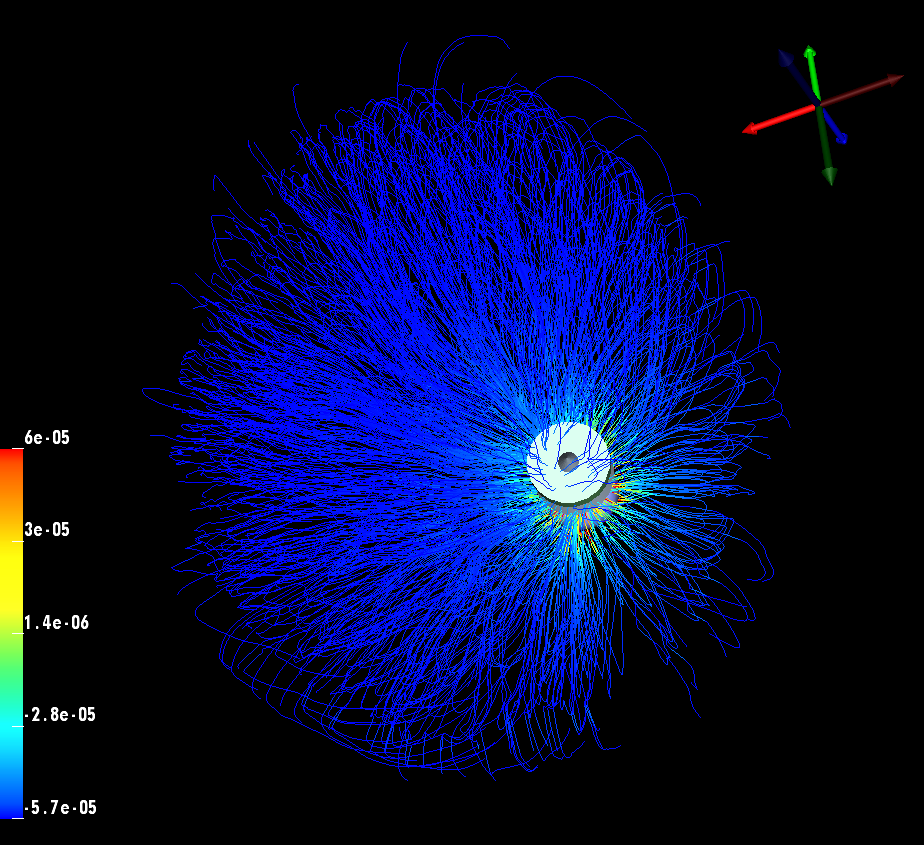
\includegraphics[width=.49\textwidth]{Figures/aniso_streamlines_top}
\caption{Anisotropic streamlines visualization with dipole source made in SCIRun}
\label{fig:anisostream}
\end{center}
\end{figure}

\begin{figure}[H]
\begin{center}
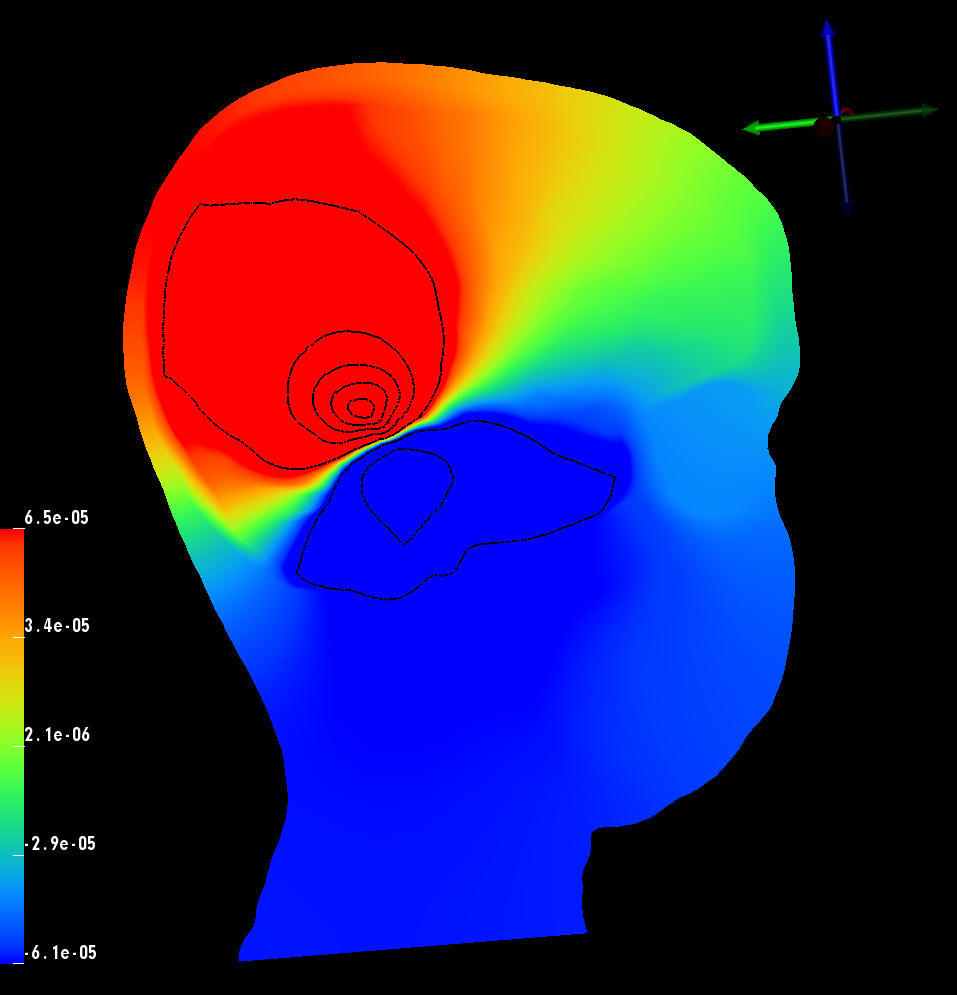
\includegraphics[width=.49\textwidth]{Figures/iso_isolines}
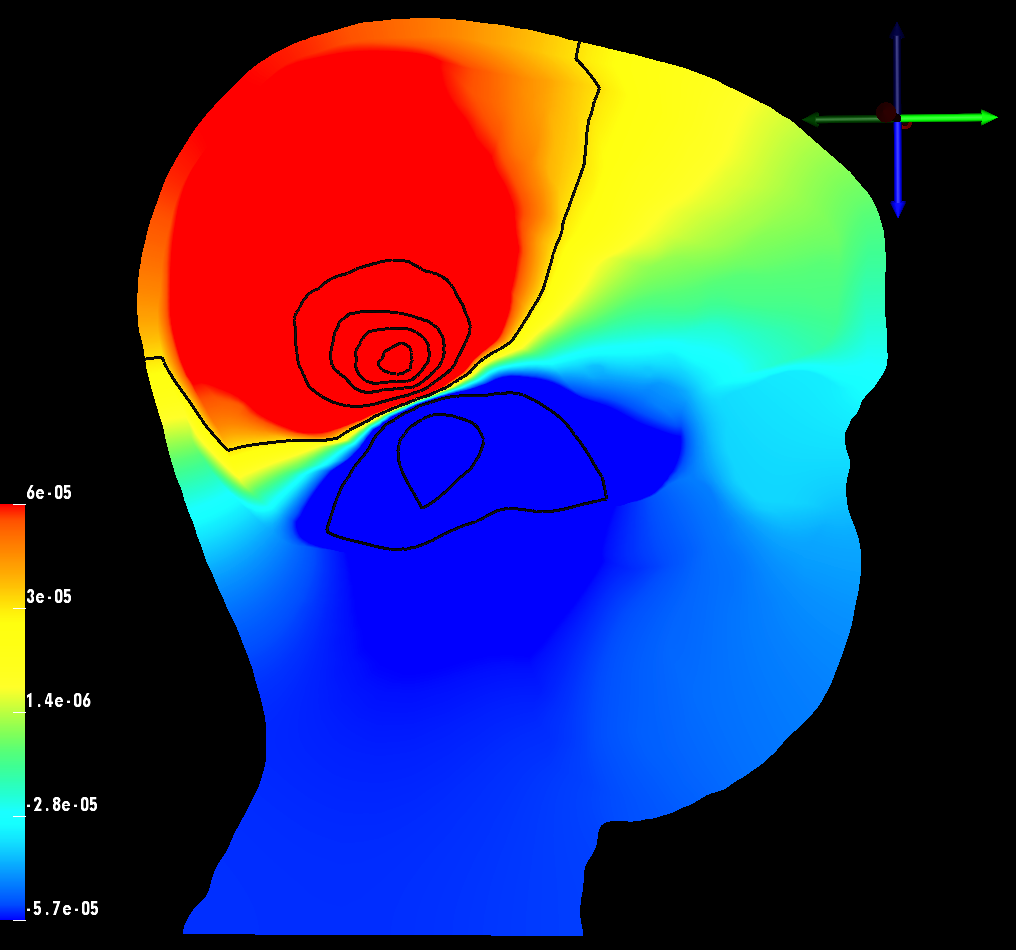
\includegraphics[width = .49\textwidth]{Figures/aniso_isolines}
\caption{Isolines comparison using SCIRun: isotropic white matter conductivity \textit{(left)}, anisotropic white matter conductivity \textit{(right)}}
\label{fig:isolines}
\end{center}
\end{figure}

\subsection{fMRI Visualization}

With the rigid and manual registration of the fMRI data to the mesh space, fMRI data was mapped properly onto the mesh (for the first time). This allows for future use of fMRI using the SCIRun package.

\begin{figure}[H]
\begin{center}
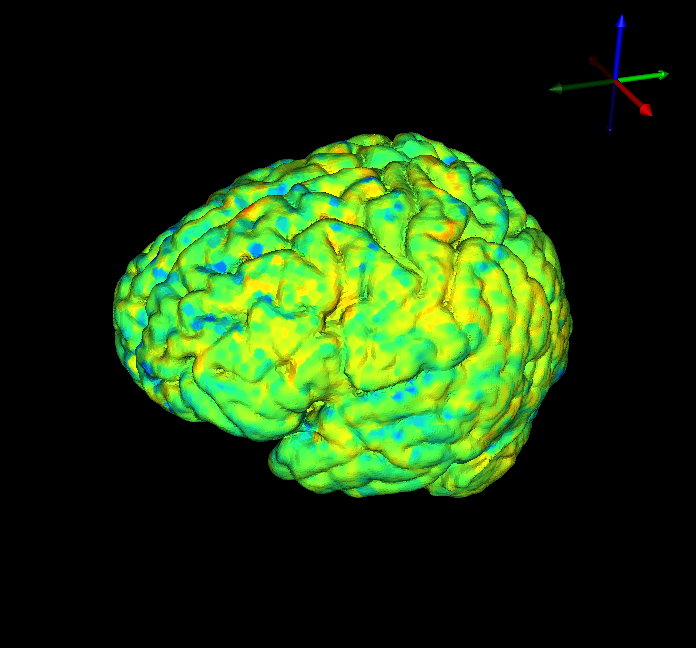
\includegraphics[width=.75\textwidth]{Figures/fmri_1}
\caption{fMRI data visualization in SCIRun: fMRI manual registration \textit{(left)} and fMRI data mapped onto cortical surface mesh \textit{(right)}}
\label{fig:fmrivis}
\end{center}
\end{figure}

\subsection{EEG Visualization}

When using EEG data, the particular application dictates what kind of additional processing, filtering, and cutting of the data needs to be done. In these visualizations it can be seen with this basic preprocessing there are bad leads, specifically around the eyes which could be due to blinking or eyes rolling, but will be improve with further specific processing.

\begin{figure}[H]
\begin{center}
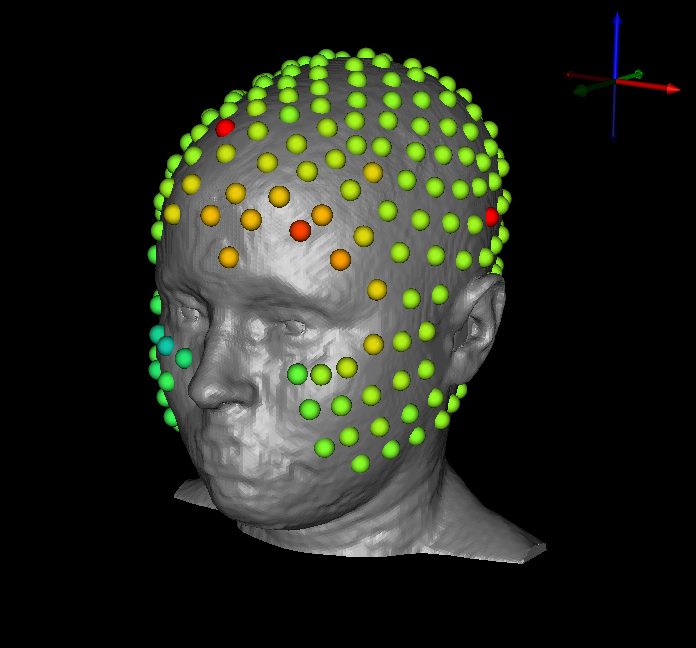
\includegraphics[width=.49\textwidth]{Figures/eeg_1}
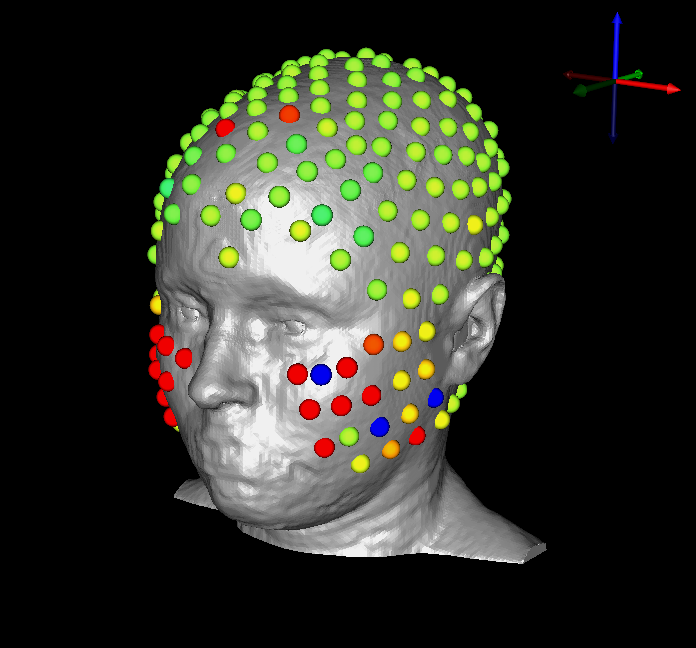
\includegraphics[width=.49\textwidth]{Figures/eeg_2}
\caption{EEG signal visualization using SCIRun. These are examples of ``bad" leads that would need further processing for specific applications}
\label{fig:eegvis}
\end{center}
\end{figure}